\documentclass{standalone}
\usepackage{tikz}
\usetikzlibrary{patterns, positioning}

\begin{document}
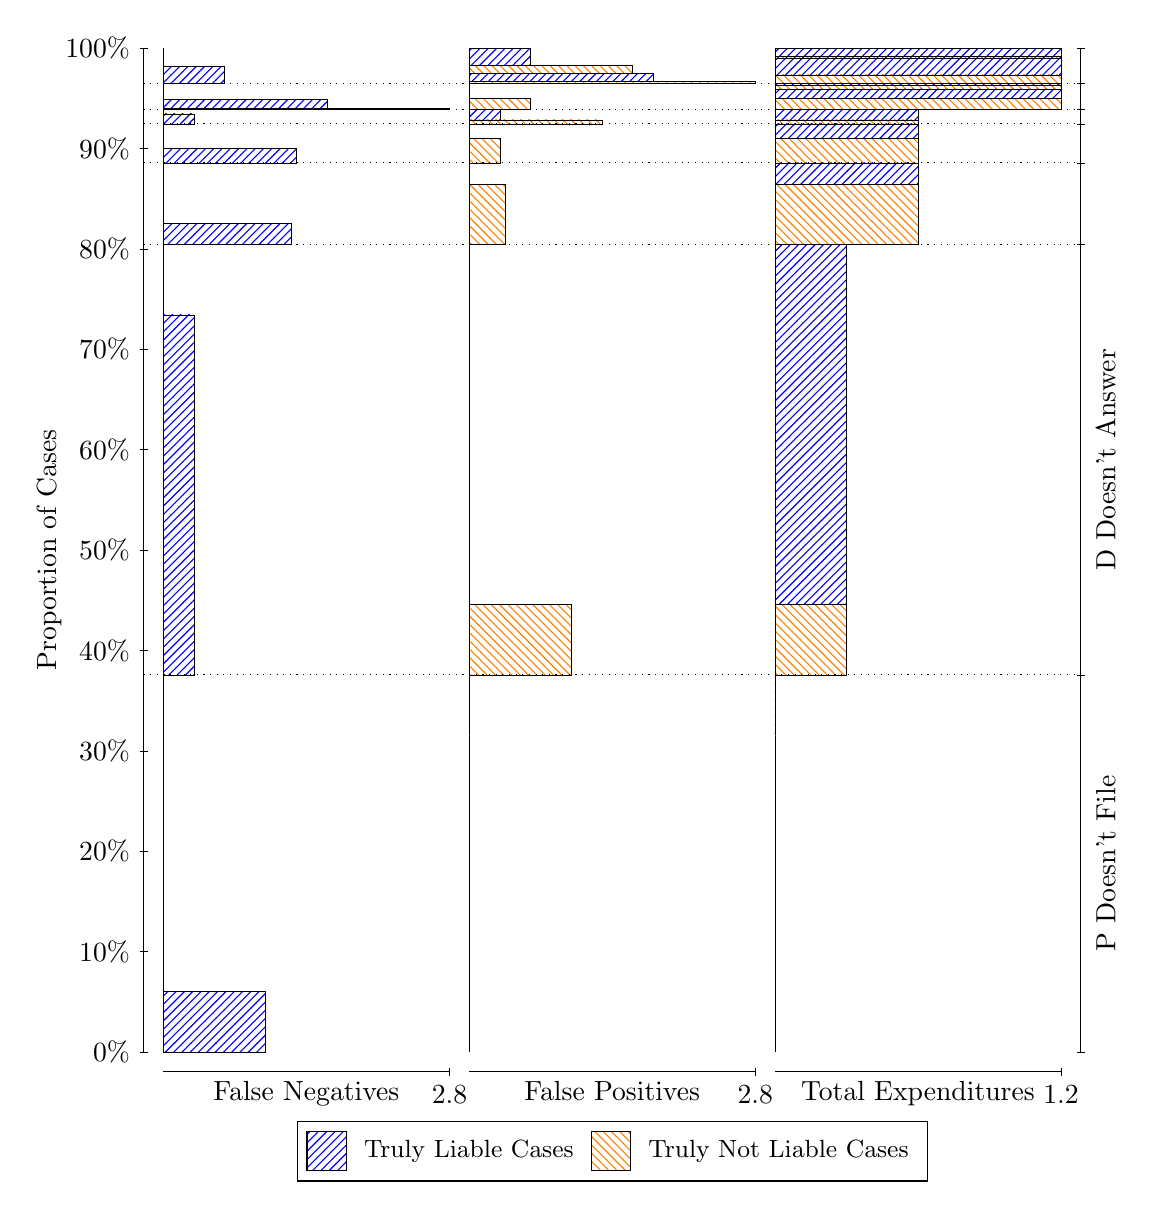
\begin{tikzpicture}
\draw[black, very thin] (1.5,1.75) -- (1.5,14.5);
\node[rotate=90, anchor=center] at (0.3, 8.125) {Proportion of Cases};
\draw[black, very thin] (1.45,1.75) -- (1.55,1.75);
\node[anchor=east] at (1.45, 1.75) {0\%};
\draw[black, very thin] (1.45,3.025) -- (1.55,3.025);
\node[anchor=east] at (1.45, 3.025) {10\%};
\draw[black, very thin] (1.45,4.3) -- (1.55,4.3);
\node[anchor=east] at (1.45, 4.3) {20\%};
\draw[black, very thin] (1.45,5.575) -- (1.55,5.575);
\node[anchor=east] at (1.45, 5.575) {30\%};
\draw[black, very thin] (1.45,6.85) -- (1.55,6.85);
\node[anchor=east] at (1.45, 6.85) {40\%};
\draw[black, very thin] (1.45,8.125) -- (1.55,8.125);
\node[anchor=east] at (1.45, 8.125) {50\%};
\draw[black, very thin] (1.45,9.4) -- (1.55,9.4);
\node[anchor=east] at (1.45, 9.4) {60\%};
\draw[black, very thin] (1.45,10.675) -- (1.55,10.675);
\node[anchor=east] at (1.45, 10.675) {70\%};
\draw[black, very thin] (1.45,11.95) -- (1.55,11.95);
\node[anchor=east] at (1.45, 11.95) {80\%};
\draw[black, very thin] (1.45,13.225) -- (1.55,13.225);
\node[anchor=east] at (1.45, 13.225) {90\%};
\draw[black, very thin] (1.45,14.5) -- (1.55,14.5);
\node[anchor=east] at (1.45, 14.5) {100\%};

\draw[black, very thin] (13.4,1.75) -- (13.4,14.5);
\draw[black, very thin] (13.35,1.75) -- (13.45,1.75);
\node[anchor=west] at (13.35, 1.75) {};
\draw[black, very thin] (13.35,6.5387) -- (13.45,6.5387);
\node[anchor=west] at (13.35, 6.5387) {};
\draw[black, very thin] (13.35,12.002) -- (13.45,12.002);
\node[anchor=west] at (13.35, 12.002) {};
\draw[black, very thin] (13.35,13.041) -- (13.45,13.041);
\node[anchor=west] at (13.35, 13.041) {};
\draw[black, very thin] (13.35,13.536) -- (13.45,13.536);
\node[anchor=west] at (13.35, 13.536) {};
\draw[black, very thin] (13.35,13.716) -- (13.45,13.716);
\node[anchor=west] at (13.35, 13.716) {};
\draw[black, very thin] (13.35,14.049) -- (13.45,14.049);
\node[anchor=west] at (13.35, 14.049) {};
\draw[black, very thin] (13.35,14.5) -- (13.45,14.5);
\node[anchor=west] at (13.35, 14.5) {};

\draw[black, very thin, pattern color=blue, pattern=north east lines] (1.75,1.75) rectangle (3.0476,2.5211);
\draw[black, very thin, pattern color=orange, pattern=north west lines] (1.75,2.5211) rectangle (1.75,6.5387);
\draw[black, very thin, pattern color=blue, pattern=north east lines] (1.75,6.5387) rectangle (2.1393,11.11);
\draw[black, very thin, pattern color=orange, pattern=north west lines] (1.75,11.11) rectangle (1.75,12.002);
\draw[black, very thin, pattern color=blue, pattern=north east lines] (1.75,12.002) rectangle (3.372,12.273);
\draw[black, very thin, pattern color=orange, pattern=north west lines] (1.75,12.273) rectangle (1.75,13.041);
\draw[black, very thin, pattern color=blue, pattern=north east lines] (1.75,13.041) rectangle (3.4369,13.224);
\draw[black, very thin, pattern color=orange, pattern=north west lines] (1.75,13.224) rectangle (1.75,13.536);
\draw[black, very thin, pattern color=blue, pattern=north east lines] (1.75,13.536) rectangle (2.1393,13.664);
\draw[black, very thin, pattern color=orange, pattern=north west lines] (1.75,13.664) rectangle (1.75,13.716);
\draw[black, very thin, pattern color=blue, pattern=north east lines] (1.75,13.716) rectangle (5.3833,13.733);
\draw[black, very thin, pattern color=blue, pattern=north east lines] (1.75,13.733) rectangle (3.8262,13.849);
\draw[black, very thin, pattern color=orange, pattern=north west lines] (1.75,13.849) rectangle (1.75,14.049);
\draw[black, very thin, pattern color=blue, pattern=north east lines] (1.75,14.049) rectangle (2.5286,14.266);
\draw[black, very thin, pattern color=orange, pattern=north west lines] (1.75,14.266) rectangle (1.75,14.398);
\draw[black, very thin, pattern color=blue, pattern=north east lines] (1.75,14.398) rectangle (1.75,14.5);
\draw[black, very thin, pattern color=orange, pattern=north west lines] (5.6333,1.75) rectangle (5.6333,5.7676);
\draw[black, very thin, pattern color=blue, pattern=north east lines] (5.6333,5.7676) rectangle (5.6333,6.5387);
\draw[black, very thin, pattern color=orange, pattern=north west lines] (5.6333,6.5387) rectangle (6.931,7.4314);
\draw[black, very thin, pattern color=blue, pattern=north east lines] (5.6333,7.4314) rectangle (5.6333,12.002);
\draw[black, very thin, pattern color=orange, pattern=north west lines] (5.6333,12.002) rectangle (6.0875,12.77);
\draw[black, very thin, pattern color=blue, pattern=north east lines] (5.6333,12.77) rectangle (5.6333,13.041);
\draw[black, very thin, pattern color=orange, pattern=north west lines] (5.6333,13.041) rectangle (6.0226,13.353);
\draw[black, very thin, pattern color=blue, pattern=north east lines] (5.6333,13.353) rectangle (5.6333,13.536);
\draw[black, very thin, pattern color=orange, pattern=north west lines] (5.6333,13.536) rectangle (7.3202,13.588);
\draw[black, very thin, pattern color=blue, pattern=north east lines] (5.6333,13.588) rectangle (6.0226,13.716);
\draw[black, very thin, pattern color=orange, pattern=north west lines] (5.6333,13.716) rectangle (6.4119,13.865);
\draw[black, very thin, pattern color=orange, pattern=north west lines] (5.6333,13.865) rectangle (5.6333,13.917);
\draw[black, very thin, pattern color=blue, pattern=north east lines] (5.6333,13.917) rectangle (5.6333,14.049);
\draw[black, very thin, pattern color=orange, pattern=north west lines] (5.6333,14.049) rectangle (9.2667,14.072);
\draw[black, very thin, pattern color=blue, pattern=north east lines] (5.6333,14.072) rectangle (7.969,14.173);
\draw[black, very thin, pattern color=orange, pattern=north west lines] (5.6333,14.173) rectangle (7.7095,14.283);
\draw[black, very thin, pattern color=blue, pattern=north east lines] (5.6333,14.283) rectangle (6.4119,14.5);
\draw[black, very thin, pattern color=orange, pattern=north west lines] (9.5167,1.75) rectangle (9.5167,5.7676);
\draw[black, very thin, pattern color=blue, pattern=north east lines] (9.5167,5.7676) rectangle (9.5167,6.5387);
\draw[black, very thin, pattern color=orange, pattern=north west lines] (9.5167,6.5387) rectangle (10.425,7.4314);
\draw[black, very thin, pattern color=blue, pattern=north east lines] (9.5167,7.4314) rectangle (10.425,12.002);
\draw[black, very thin, pattern color=orange, pattern=north west lines] (9.5167,12.002) rectangle (11.333,12.77);
\draw[black, very thin, pattern color=blue, pattern=north east lines] (9.5167,12.77) rectangle (11.333,13.041);
\draw[black, very thin, pattern color=orange, pattern=north west lines] (9.5167,13.041) rectangle (11.333,13.353);
\draw[black, very thin, pattern color=blue, pattern=north east lines] (9.5167,13.353) rectangle (11.333,13.536);
\draw[black, very thin, pattern color=orange, pattern=north west lines] (9.5167,13.536) rectangle (11.333,13.588);
\draw[black, very thin, pattern color=blue, pattern=north east lines] (9.5167,13.588) rectangle (11.333,13.716);
\draw[black, very thin, pattern color=orange, pattern=north west lines] (9.5167,13.716) rectangle (13.15,13.865);
\draw[black, very thin, pattern color=blue, pattern=north east lines] (9.5167,13.865) rectangle (13.15,13.98);
\draw[black, very thin, pattern color=orange, pattern=north west lines] (9.5167,13.98) rectangle (13.15,14.032);
\draw[black, very thin, pattern color=blue, pattern=north east lines] (9.5167,14.032) rectangle (13.15,14.049);
\draw[black, very thin, pattern color=orange, pattern=north west lines] (9.5167,14.049) rectangle (13.15,14.159);
\draw[black, very thin, pattern color=blue, pattern=north east lines] (9.5167,14.159) rectangle (13.15,14.376);
\draw[black, very thin, pattern color=orange, pattern=north west lines] (9.5167,14.376) rectangle (13.15,14.398);
\draw[black, very thin, pattern color=blue, pattern=north east lines] (9.5167,14.398) rectangle (13.15,14.5);
\draw[black, dotted] (1.5,6.5387) -- (13.4,6.5387);
\draw[black, dotted] (1.5,12.002) -- (13.4,12.002);
\draw[black, dotted] (1.5,13.041) -- (13.4,13.041);
\draw[black, dotted] (1.5,13.536) -- (13.4,13.536);
\draw[black, dotted] (1.5,13.716) -- (13.4,13.716);
\draw[black, dotted] (1.5,14.049) -- (13.4,14.049);
\draw[black, very thin] (1.75,1.5) -- (5.3833,1.5);
\node[anchor=north] at (3.5667, 1.5) {False Negatives};
\draw[black, very thin] (5.3833,1.45) -- (5.3833,1.55);
\node[anchor=north] at (5.3833, 1.45) {2.8};

\draw[black, very thin] (5.6333,1.5) -- (9.2667,1.5);
\node[anchor=north] at (7.45, 1.5) {False Positives};
\draw[black, very thin] (9.2667,1.45) -- (9.2667,1.55);
\node[anchor=north] at (9.2667, 1.45) {2.8};

\draw[black, very thin] (9.5167,1.5) -- (13.15,1.5);
\node[anchor=north] at (11.333, 1.5) {Total Expenditures};
\draw[black, very thin] (13.15,1.45) -- (13.15,1.55);
\node[anchor=north] at (13.15, 1.45) {1.2};

\node[black, centered, rotate=90] at (13.72, 4.1444) {P Doesn't File};
\node[black, centered, rotate=90] at (13.72, 9.2706) {D Doesn't Answer};






\draw (7.449999999999999,1.5) node[draw=none] (baseCoordinate) {};
\begin{scope}[align=center]
        \matrix[scale=0.5, draw=black, below=0.5cm of baseCoordinate, nodes={draw}, column sep=0.1cm]{
            \node[rectangle, draw, minimum width=0.5cm, minimum height=0.5cm, pattern=north east lines, pattern color=blue] {}; &
            \node[draw=none, font=\small] (B) {Truly Liable Cases}; &
            \node[rectangle, draw, minimum width=0.5cm, minimum height=0.5cm, pattern=north west lines, pattern color=orange] {}; &
            \node[draw=none, font=\small] (B) {Truly Not Liable Cases}; \\
            };
\end{scope}

\end{tikzpicture}
\end{document}